\section{Methods}

In researching for this paper, more often than not, we found that, while
the core concepts weren't too difficult to get our heads around, the
higher-level explanations would often go right over our heads.

We identified two attributes that mattered most when implementing vertex
cover (or any graph-theoretic) algorithm. These two attributes, size and
source, each bubble down to two sub-cases.

Size:

\begin{itemize}
    \item
          In-memory - The graph is small enough to store within memory. This
          means that actions can be performed on the graph taking in account the
          entire graph.
    \item
          Out-of-memory - The graph is too large to store within memory in it's
          entirety. Actions must now be made on small parts of the graph without
          the knowledge of other parts.
\end{itemize}

Source:

\begin{itemize}
    \item
          Local - One has direct access to the graph, for example, in the form
          of a file.
    \item
          Networked - One does not have direct access, the data is streamed to
          you in pieces. This may be either due to the size of the data (it
          being too large to store feasibly) or due to the nature of the data.
          This nature being that the data could be fragmented across databases
          and so must be pre-processed in some way to put it all together.
\end{itemize}

This allows us to break down our aims into three sections based on these
attributes. For in-memory sized local graphs (the traditional setting)
we're able to provide traditional tools. This includes visualisations
and simplified implementations using well-worn graph libraries. In this
setting we can simulate streaming by looping through the edges of a
graph. This gives us a particular advantage in seeing truly how the
algorithms work as we are able to see the entire graph at the same time.

The second section is for out-of-memory sized local graphs. In our
original plan, this section didn't exist as we assumed most
implementation details would come forward when implementing into a real
streaming framework. However, we found that this was too much of a jump
so this middle step was envisioned to allow for a true streaming
implementation while still being in the familiarity of the core Python
libraries. So that's exactly what we'll be doing. Having the graph
represented by an edge list stored in a file allows us to read from the
file line-by-line and therefore edge-by-edge. This is exactly how a
streaming application would see the input of a graph. Since the time
taken to read from a file is negligible in comparison to any network
activity, we will be able to gauge the performance of these algorithms
with minimal external variables. This gives us a platform for accurate
performance profiling.

The final section is for out-of-memory sized networked graphs. This is
what you'd consider to be an actual use case. This is the most flexible
section, in that, there are many ways of going about it depending on
your situation. We're taking this as an opportunity to build a
proof-of-concept system that covers the basics. Apache Kafka has shown
promise in it's versatility as a streaming platform [citation needed] rather than being
tied down to a particular workflow. This allows for our fairly custom
implementation of stream processing. Most streaming platforms prioritise
parallelisation in their processing which we don't concern ourselves
with. Our data source will be external in the sense that it could be
replicated to run on a server far, far away but for ease of development
sake it will be ran locally.

\subsection{The Algorithms}

\subsubsection{Branching - Classical}

Bounded Search Trees have been used to solve many parameterized problems
due to their bounded nature. Starting with the whole graph, this version
works by recursively branching on each edge, deleting a chosen vertex
along the way. If you have an empty graph before you reach a depth of
\(k\) then you will have your vertex cover. If not, then you simply try
every other path down the tree, choosing a different set of vertices on
each path. If none of the paths work out then you can conclude that no
vertex cover exists with a maximum size of \(k\).

\begin{algorithm}[H]
    \caption{Branching - Classical}
    \DontPrintSemicolon
    \SetKwFunction{FBranching}{branching}
    \SetKwFunction{FEdges}{numberOfEdges}
    \SetKwFunction{FCopy}{copy}
    \SetKwFunction{FFirstEdge}{firstEdge}
    \SetKwFunction{FRemoveNode}{removeNode}
    \SetKwFunction{FAdd}{add}

    \KwInput{Graph $graph$ to calculate vertex cover on}
    \KwInput{Value $k$ for maximum size of vertex cover}
    \KwOutput{Vertex cover of maximum size $k$ if one exists}
    \Func{\FBranching{graph\textnormal{: Graph, }k\textnormal{: int, }vertexCover\textnormal{: set}}}{
        \If{\FEdges{graph} $= 0$}{
            \Return vertexCover
        }
        \If{k $= 0$}{
            \Return Null
        }
        $u, v \gets$ \FFirstEdge{graph}\;
        \tcp{Run recursively on left side}
        $leftGraph \gets$ \FCopy{graph}\;
        \FRemoveNode{leftGraph, u}\;
        $leftVertexCover \gets$ \FCopy{vertexCover}\;
        \FAdd{leftVertexCover, u}\;
        $leftVertexCover \gets$ \FBranching{leftGraph, k - 1, leftVertexCover}\;

        \If{leftVertexCover \KwIs \KwNot Null}{
            \Return leftVertexCover
        }

        \tcp{Run recursively on right side}
        $rightGraph \gets$ \FCopy{graph}\;
        \FRemoveNode{rightGraph, u}\;
        $rightVertexCover \gets$ \FCopy{vertexCover}\;
        \FAdd{rightVertexCover, u}\;
        $rightVertexCover \gets$ \FBranching{rightGraph, k - 1, rightVertexCover}\;
        \Return rightVertexCover
    }

\end{algorithm}

Being a search tree, it is noted that this algorithm can be tweaked to
be a breadth-first search rather than depth-first. This will prioritise
the search for a minimum vertex cover which may be more useful in some
situations.

\subsubsection{Branching - Stream}

\cite{chitnis2019towards} converted the above branching
algorithm into one that was compatible with the streaming model. This
algorithm required \(O(k\cdot \log n)\) space and \(2^k\) passes. We
noticed their pseudocode had an error. In their version, if the end of
the edge stream (\(j\) in their pseudocode) was reached before a depth
(\(i\) in their pseudocode) of \(k\) was reached then the program would
presumably throw an exception as there were no more edges to read. This
is due to the fact that the check for whether the end of the stream had
been reached was put outside the inner-most loop. Below is our corrected
version.

\begin{verbatim}
    while X != END do
        S = theta, i = 1, j = 1
        while i != k + 1 do
            Let e_j = u - v such that u < v under the ordering sigma
            if Both u not in S and v not in S then
                if X[i] = 0 then S ← S U {u}
                else S ← S U {v}
                i ← i + 1
            j ← j + 1
            if j = m + 1 then Return S and abort
        X ← Dictk(Next(X))
    if X = END then Return NO
\end{verbatim}

In implementing this algorithm, we found that the way the pseudocode had
been structured made implementation difficult. This is because streaming
platforms such as Kafka rely on brokers recording whether they have seen
a message or not; this is counted as the number of \texttt{acks}
(acknowledgements). If the algorithm were to exit before acknowledging
all the edges in the stream, then these edges would lay dormant until
another algorithm was run and it would start reading them erroneously.
This caused us to rewrite the algorithm with the inner-most loop being
based on looping through the edges rather than looping through the
depths of the tree.

change this explanation a little to take out Kafka

\begin{algorithm}[H]
    \caption{Branching - Stream}
    \DontPrintSemicolon
    \SetKwFunction{FCalculateVC}{calculateVC}
\end{algorithm}

\subsubsection{Kernelization - Classical}

First devised by \cite{buss1991nondeterminism}, given an input of an
undirected graph \(G\) and a number \(k\), this algorithm works by
applying the following rules until no more reductions can be made.

\begin{enumerate}
    \item
          If \(k > 0\) and \(v\) is a vertex of degree \(> k\), remove \(v\)
          from the graph and decrease the value of \(k\) by 1.
    \item
          If \(v\) is an isolated vertex, remove it.
    \item
          If more than \(k^2\) \sout{edges remain in the graph, and neither of
              the previous two rules can be applied, then the graph cannot contain a
              vertex cover of size \(k\).} reword this
\end{enumerate}

reword this

\sout{The output is a set of at most \(k\) vertices that includes an
    endpoint of every edge in the graph, if such a set exists, or a failure
    exception if no such set exists.} This is the first \(O(k^2)\)
vertices kernel. This was then improved upon in
\cite{balasubramanian1998improved} but for the sake of this paper we will
be using the simpler Buss kernelization algorithm.

\begin{verbatim}
    vertex_cover ← empty
    while True
        reduction ← False
        foreach node in graph.nodes
            if k > 0 and node.degree > k:
                reduction ← True
                graph ← graph - node
                vertex_cover ← vertex_cover U {node}
                k ← k - 1
            else if node.degree = 0
                reduction ← True
                graph ← graph - node

        if reduction = False
            break

    if kernel.number_of_edges() > k^2:
        return null

    return graph
\end{verbatim}

\begin{algorithm}[H]
    \caption{Kernelization - Non-Stream}
    \DontPrintSemicolon
    \SetKwFunction{FKernelize}{kernelize}
    \SetKwFunction{FCopy}{copy}
    \SetKwFunction{FDegree}{degree}

    \KwInput{Graph $graph$ to calculate vertex cover on}
    \KwInput{Value $k$ for maximum size of vertex cover}
    \KwOutput{Kernel of graph and vertex cover}
    \Func{\FKernelize{graph\textnormal{: Graph, }k\textnormal{ : int}}}{
        $kernel \gets$ \FCopy{graph}\;
        $vertexCover$ : set\;
        $reductionsCanBeMade \gets$ True\;
        \While{reductionsCanBeMade}{
            $reductionMade \gets$ False\;
            \For{$node$ \KwIn $kernel$.nodes}{
                \uIf{k > $0$ \KwAnd \FDegree{node} > k}{
                    $reductionMade \gets$ False\;
                    $kernel$.removeNode($node$)\;
                    $vertexCover$.add($node$)\;
                    $k \gets k - 1$\;
                }
                \ElseIf{\FDegree{node} = 0}{
                    $kernel$.removeNode($node$)\;
                }
            }
            \If{\KwNot reductionMade}{
                $reductionsCanBeMade \gets$ False\;
            }
        }
        \Return kernel, vertexCover\;
    }
\end{algorithm}

\subsubsection{Kernelization - Stream}

\cite{chitnis2015parameterized} developed this algorithm. It
works by greedily maintaining a maximal matching and for each matched
vertex \(v\), keeping up to k edges incident on \(v\). If at any point
the number of matched edges exceeds \(k\) then we can conclude no such
vertex cover exists of size \(\leq k\) and end the stream. If we reach
the end of the stream then a kernel consisting of all the matched edges
and their neighbours is returned. The space complexity of this algorithm
is \(O(k^2)\).

\begin{verbatim}
    kernel = Kernel(k)
    kernel_exists = True
    maximal_matching = {}
    for u, v in stream
        is_neighbour = False
        if u is in maximal_matching
            is_neighbour = True
            matched_edge, neighbours = maximal_matching.get_match(u)
            vertex_pos = matched_edge.index(u)
            if len(neighbours[vertex_pos]) < k
                neighbours[vertex_pos].append((u, v))

        else if v is in maximal_matching
            is_neighbour = True
            matched_edge, neighbours = maximal_matching.get_match(v)
            vertex_pos = matched_edge.index(v)
            if len(neighbours[vertex_pos]) < self.k
                neighbours[vertex_pos].append((u, v))

        if not is_neighbour
            maximal_matching.add((u, v))

            if len(maximal_matching) > k
                return null

    return kernel
\end{verbatim}

\begin{algorithm}[H]
    \caption{Kernelization - Stream}
    \DontPrintSemicolon
    \SetKwFunction{FInit}{init}
    \SetKwFunction{FNext}{next}
    \SetKwFunction{FNeighbours}{neighbours}
    \SetKwFunction{FLen}{length}

    \KwInput{Edges $u$, $v$ from a stream}
    \KwInput{Value $k$ for maximum size of vertex cover}
    \KwOutput{Boolean whether kernel exists}
    \KwData{$k$, $matchings$}
    \Func{\FInit{k\textnormal{: int}}}{
        $k$ : int $\leftarrow$ $k$\;
        $matchings$ : dict\;
    }
    \Func{\FNext{u, v}}{
        $isNeighbour$ : bool $\gets$ False\;
        \If{u $\KwIs$ $\KwIn$ matchings $\KwAnd$ $\FLen{\FNeighbours{u}}$ $\leq$ k}{
            matchings$[u]$.append((u,v))\;
            isNeighbour $\gets$ True\;
        }
        \If{v $\KwIs$ $\KwIn$ matchings $\KwAnd$ $\FLen{\FNeighbours{v}}$ $\leq$ k}{
            $matchings[v]$.append($(u,v)$)\;
            $isNeighbour$ $\gets$ True\;
        }
        \If{$\KwNot$ $isNeighbour$}{
            $matchings$.append((u,v))\;
            \If{$\FLen{matchings}$ $>$ k}{
                \Return False\;
            }
        }
        \Return True\;
    }
\end{algorithm}

\subsection{Local - Visualisation}

This is the traditional case. The graph is small enough to use in-memory
and you have local access to it, so you are able to use which ever tools
you wish to calculate the vertex cover. We will be using a library
called NetworkX \cite{hagberg2008exploring}. NetworkX provides data structures
for graphs with an intuitive API. It also includes a module for drawing
graphs with Matplotlib \cite{hunter2007matplotlib}, a Python visualization
library that has been around since 2003 [citation needed]. With these tools we will be
able to create programs that create visualisations of both the
kernelization and branching stream algorithms.

There are some key aspects we'd like to highlight in both algorithms.
For the kernelization algorithm, these include being able to compare the
kernel to the whole graph and being able to see when edges are not added
to the kernel. For the branching algorithm, these include the binary
string and the binary search tree.


\subsection{Local-Stream - Performance Benchmarking}

In this case the graph is no longer large enough to store in-memory but
you are able to have direct access to it. The graph may be large but it
is feasible to store the graph on disk since disk sizes are often many
magnitudes larger than that of memory. Traditional algorithms are no
longer applicable here, this is the first example where the invention of
streaming algorithms is a necessity.

\subsubsection{Datasets}

While the original intention for this section of the project was to test
against large graphs from all possible backgrounds
(constructed/synthetic/real), we quickly realised that many, if not all,
graphs we considered were of the same shape/form. That is, they all had
relatively uniform density and so had a minimum vertex cover close to
the number of vertices. In order to get any results that was anything
more than a null result, we would have to generate some graphs of our
own. These graphs would have to have a large number of edges while
simultaneously having a low vertex cover number. This leads to graphs
with a low level of connectivity.

Eventually you get to a point when the datasets become too large to even
read.

\begin{figure}[htb]
    \centering
    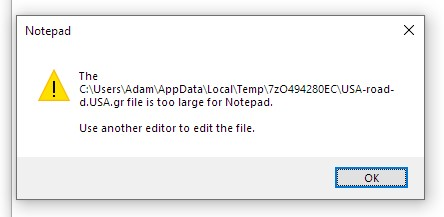
\includegraphics{dataset-too-big.jpg}
    \caption{Dataset too big 1}
\end{figure}

Visual Studio Code, a more modern text editor, is able to open the file
however not without performance issues even when wrapping and folding
have been turned off.

\begin{figure}[htb]
    \centering
    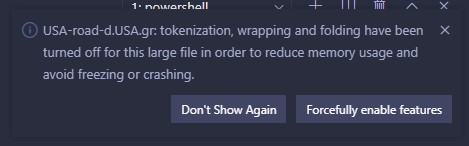
\includegraphics{dataset-too-big3.jpg}
    \caption{Dataset too big 3}
\end{figure}

There is even a limit for Visual Studio Code though.

\begin{figure}[htb]
    \centering
    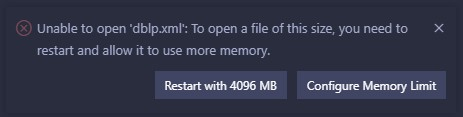
\includegraphics{dataset-too-big2.jpg}
    \caption{Dataset too big 2}
\end{figure}

\subsubsection{Testing and Comparison}

We don't live in a world anymore where we have to hack our way around
machines to push the limits of their memory just so we can play some
games. We haven't for a while. This goes the same for algorithms. Most
of the time, we will happily sacrifice memory efficiency for any extra
pittance of time efficiency. Memory is dispensable, our time is not.
This may still be true for streaming algorithms, but only to an extent.
We are very much interested in both time and space complexity here. And
so, we need to test as such.

For memory profiling, we will use the Python package
\texttt{memory-profiler} which records memory usage at intervals of
\(0.1\text{s}\). It also allows for tagging of functions meaning that we
can see when each function starts and ends. Creating a script to run
both the local and stream versions of each algorithm allowed us to show
the memory usage of each side by side.

For runtime analysis, we will use a Python package called
\texttt{pyperf}. It includes tools for writing, running, and analysing
runtime benchmarks. By creating a script to run through a handful of
graphs and \(k\) values and run them with both the local and stream
versions of each algorithm, we should be able to paint a clearer picture
of how the stream versions compare to their local counterparts.

\subsection{Stream - Implementation}

This is the main case. In a typical situation, knowledge of the graph's
attributes will be limited so it should be treated as an unbounded
stream (a stream that has no end). The opposite of this would be
treating it as a bounded stream, where we know there is an end to the
stream.

\subsubsection{Batch vs Stream processing}

Most ``streaming'' applications work on \textbf{unbounded} streams.
These are data streams which are essentially infinite. Examples include:
sensor readings and application logging. In these cases, the objective
is not to obtain a final result but to aggregate the data before storing
it for future use. This would be classed as \textbf{stream processing}.

Our problem of Vertex Cover would be classed as \textbf{batch
    processing}. We may be working on a data stream but once either
algorithm has completed we won't need to run it again.

Most streaming platforms (especially those in the Apache line up) work
on unbounded stream processing. So finding a streaming platform
appropriate for batch processing was a little more tricky. There are a
number of ``graph'' processing frameworks.

Streaming platforms are the base on which a data stream is sent and
received. Examples include:

\begin{itemize}
    \item
          Apache Kafka
    \item
          Amazon Kinesis
    \item
          Apache Spark Streaming
    \item
          Google Cloud Pub/Sub
    \item
          Google Cloud DataFlow
    \item
          RabbitMQ
\end{itemize}

Once we have the platform we need an in-memory framework to handle the
processing of each item in the stream. This is where the algorithms will
actually run. There are a whole number of frameworks for this, all of
which have their own niche use cases. Examples include:

\begin{itemize}
    \item
          Apache Spark
    \item
          Apache Spark GraphX
    \item
          Apache Flink
    \item
          Apache Beam
    \item
          Apache Samza
\end{itemize}

\subsubsection{In-memory sized stream graphs}

If you know beforehand the size of the graph and it's of an in-memory
size then you don't need to go through the hassle of treating it as a
stream. One pass through the graph will allow you to store the graph
locally and therefore be able to use it as a local graph instead.

\subsubsection{Actors}


\begin{itemize}
    \item
          producer - explain role and abstract interface
\end{itemize}